\documentclass[tikz,border=6pt]{standalone}
% Shared style for the HERMESS schematic figures (compiled by build.sh).
% ETH palette; Latin Modern (the LaTeX default) to match the documentation.
\usepackage{amsmath}
\usepackage{tikz}
\usetikzlibrary{arrows.meta,positioning,calc,shapes.geometric,circuits.ee.IEC}
\definecolor{ethblue}{HTML}{215CAF}
\definecolor{ethpetrol}{HTML}{007894}
\definecolor{ethgrey}{HTML}{6F6F6F}
\tikzset{
  block/.style      = {draw=ethblue, thick, fill=ethblue!8, minimum height=9mm,
                       minimum width=16mm, inner sep=2.5pt, align=center},
  sum/.style        = {draw=ethblue, thick, circle, fill=white, minimum size=4.5mm, inner sep=0pt},
  sig/.style        = {-{Latex[length=2.4mm]}, thick},
  wire/.style       = {thick},
  node distance     = 9mm and 12mm,
  every node/.style = {font=\small},
  lbl/.style        = {font=\small, inner sep=1.5pt},
  port/.style       = {font=\small\itshape, text=ethgrey},
}

\begin{document}
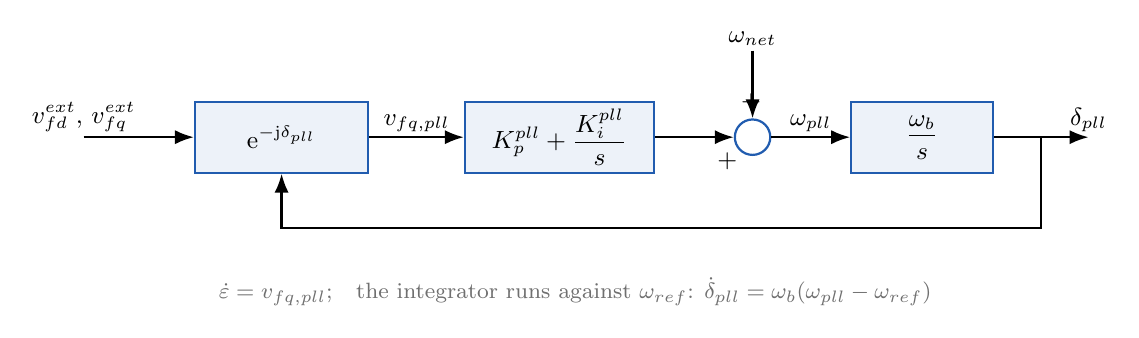
\begin{tikzpicture}
  \node[block, minimum width=22mm] (rot) {$\mathrm{e}^{-\mathrm{j}\delta_{pll}}$};
  \node[block, right=12mm of rot, minimum width=24mm] (pi) {$K_p^{pll} + \dfrac{K_i^{pll}}{s}$};
  \node[sum, right=10mm of pi] (s) {};
  \node[lbl] at ($(s)+(-0.02,0.44)$) {$+$};
  \node[lbl] at ($(s)+(-0.32,-0.30)$) {$+$};
  \node[block, right=10mm of s, minimum width=18mm] (int) {$\dfrac{\omega_b}{s}$};
  \draw[sig] ($(rot.west)+(-1.4,0)$) node[above, lbl] {$v_{fd}^{ext},\, v_{fq}^{ext}$} -- (rot);
  \draw[sig] (rot) -- (pi) node[midway, above, lbl] {$v_{fq,pll}$};
  \draw[sig] (pi) -- (s);
  \draw[sig] ($(s)+(0,1.1)$) node[above, lbl] {$\omega_{net}$} -- (s);
  \draw[sig] (s) -- (int) node[midway, above, lbl] {$\omega_{pll}$};
  \draw[sig] (int.east) -- ++(1.2,0) node[above, lbl] {$\delta_{pll}$};
  \draw[sig] ($(int.east)+(0.6,0)$) -- ++(0,-1.15) -| ($(rot.south)+(0,0)$);
  \node[lbl, text=ethgrey] at ($(pi.south)+(0.2,-1.5)$)
    {\footnotesize $\dot{\varepsilon} = v_{fq,pll}$;\quad the integrator runs against $\omega_{ref}$: $\dot{\delta}_{pll} = \omega_b(\omega_{pll} - \omega_{ref})$};
\end{tikzpicture}
\end{document}
